\documentclass[a4paper,14pt, unknownkeysallowed]{extreport}

\usepackage{cmap} % Улучшенный поиск русских слов в полученном pdf-файле
\usepackage[T2A]{fontenc} % Поддержка русских букв
\usepackage[utf8]{inputenc} % Кодировка utf8
\usepackage[english,russian]{babel} % Языки: русский, английский
%\usepackage{pscyr} % Нормальные шрифты
\usepackage{enumitem}

\usepackage[14pt]{extsizes}

\usepackage{caption}
\captionsetup{labelsep=endash}
\captionsetup[figure]{name={Рисунок}}

\usepackage{amsmath}

\usepackage{geometry}
\geometry{left=30mm}
\geometry{right=15mm}
\geometry{top=20mm}
\geometry{bottom=20mm}

\usepackage{titlesec}
\titleformat{\section}
	{\normalsize\bfseries}
	{\thesection}
	{1em}{}
\titlespacing*{\chapter}{0pt}{-30pt}{8pt}
\titlespacing*{\section}{\parindent}{*4}{*4}
\titlespacing*{\subsection}{\parindent}{*4}{*4}

\usepackage{setspace}
\onehalfspacing % Полуторный интервал

\frenchspacing
\usepackage{indentfirst} % Красная строка

\usepackage{titlesec}
\titleformat{\chapter}{\LARGE\bfseries}{\thechapter}{20pt}{\LARGE\bfseries}
\titleformat{\section}{\Large\bfseries}{\thesection}{20pt}{\Large\bfseries}

\usepackage{listings}
\usepackage{xcolor}

% Для листинга кода:
\lstset{ %
	language=c++,   					% выбор языка для подсветки	
	basicstyle=\small\sffamily,			% размер и начертание шрифта для подсветки кода
	numbers=left,						% где поставить нумерацию строк (слева\справа)
	%numberstyle=,					% размер шрифта для номеров строк
	stepnumber=1,						% размер шага между двумя номерами строк
	numbersep=5pt,						% как далеко отстоят номера строк от подсвечиваемого кода
	frame=single,						% рисовать рамку вокруг кода
	tabsize=4,							% размер табуляции по умолчанию равен 4 пробелам
	captionpos=t,						% позиция заголовка вверху [t] или внизу [b]
	breaklines=true,					
	breakatwhitespace=true,				% переносить строки только если есть пробел
	escapeinside={\#*}{*)},				% если нужно добавить комментарии в коде
	backgroundcolor=\color{white},
}

\usepackage{pgfplots}
\usetikzlibrary{datavisualization}
\usetikzlibrary{datavisualization.formats.functions}

\usepackage{graphicx}
\newcommand{\img}[3] {
	\begin{figure}[h!]
		\center{\includegraphics[height=#1]{inc/img/#2}}
		\caption{#3}
		\label{img:#2}
	\end{figure}
}
\newcommand{\boximg}[3] {
	\begin{figure}[h]
		\center{\fbox{\includegraphics[height=#1]{inc/img/#2}}}
		\caption{#3}
		\label{img:#2}
	\end{figure}
}

\usepackage[justification=centering]{caption} % Настройка подписей float объектов

\usepackage[unicode,pdftex]{hyperref} % Ссылки в pdf
\hypersetup{hidelinks}

\usepackage{csvsimple}



\newcommand{\code}[1]{\texttt{#1}}

\begin{document}


\begin{titlepage}
	\newgeometry{pdftex, left=2cm, right=2cm, top=2.5cm, bottom=2.5cm}
	\fontsize{12pt}{12pt}\selectfont
	\noindent \begin{minipage}{0.15\textwidth}
		
\includegraphics[width=\linewidth]{img/logo.jpg}
	\end{minipage}
	\noindent\begin{minipage}{0.9\textwidth}\centering
		\textbf{Министерство науки и высшего образования Российской Федерации}\\
		\textbf{Федеральное государственное бюджетное образовательное учреждение высшего образования}\\
		\textbf{«Московский государственный технический университет имени Н.~Э.~Баумана}\\
		\textbf{(национальный исследовательский университет)»}\\
		\textbf{(МГТУ им. Н.~Э.~Баумана)}
	\end{minipage}
	
	\noindent\rule{18cm}{3pt}
	\newline\newline
	\noindent ФАКУЛЬТЕТ $\underline{\text{«Информатика и системы управления»~~~~~~~~~~~~~~~~~~~~~~~~~~~~~~~~~~~~~~~~~~~~~~~~~~~~~~~}}$ \newline\newline
	\noindent КАФЕДРА $\underline{\text{«Программное обеспечение ЭВМ и информационные технологии»~~~~~~~~~~~~~~~~~~~~~~~}}$\newline\newline\newline\newline\newline\newline\newline
	

	\begin{center}
  		\noindent\begin{minipage}{1.3\textwidth}\centering
  		\Large\textbf{   Отчет по лабораторной работе № 5}\newline
  		\textbf{по дисциплине "Анализ алгоритмов"}\newline\newline\newline
  		\end{minipage}
	\end{center}
	
	\noindent\textbf{Тема} $\underline{\text{~~Конвейерная обработка данных~~~~~~~~~~~~~~~~~~~~~~~~~~~~~~~~~~~~~~~~~~~~~~~~~~~~~~~~~~~~~~~~~~~~~}}$\newline\newline\newline
	\noindent\textbf{Студент} $\underline{\text{~~Хамзина Р. Р.~~~~~~~~~~~~~~~~~~~~~~~~~~~~~~~~~~~~~~~~~~~~~~~~~~~~~~~~~~~~~~~~~~~~~~~~~~~~~~~~~~~~~~~~~}}$\newline\newline
	\noindent\textbf{Группа} $\underline{\text{~~ИУ7-53Б~~~~~~~~~~~~~~~~~~~~~~~~~~~~~~~~~~~~~~~~~~~~~~~~~~~~~~~~~~~~~~~~~~~~~~~~~~~~~~~~~~~~~~~~~~~~~~~~~}}$\newline\newline
	\noindent\textbf{Оценка (баллы)} $\underline{\text{~~~~~~~~~~~~~~~~~~~~~~~~~~~~~~~~~~~~~~~~~~~~~~~~~~~~~~~~~~~~~~~~~~~~~~~~~~~~~~~~~~~~~~~~~~~~~~~~~~}}$\newline\newline
	\noindent\textbf{Преподаватель} $\underline{\text{~~Волкова Л. Л.~~~~~~~~~~~~~~~~~~~~~~~~~~~~~~~~~~~~~~~~~~~~~~~~~~~~~~~~~~~~~~~~~~~~~~~~~~~~~~}}$\newline
	
	\begin{center}
		\vfill
		Москва~---~\the\year
		~г.
	\end{center}
	\restoregeometry
\end{titlepage}


\tableofcontents
\setcounter{page}{2}
\chapter*{Введение}
\addcontentsline{toc}{chapter}{Введение}

Одной из задач программирования является ускорение решения вычислительных задач. Один из способов ее решения - использование параллельных вычислений.

В последовательном алгоритме решения какой-либо задачи есть операции, которые может выполнять только один процесс, например, операции ввода и вывода. Кроме того, в алгоритме могут быть операции, которые могут выполняться параллельно разными процессами. Алгоритм, операции которого могут быть выполнены разными процессами параллельно, называют параллельным. Каждый процесс состоит из одного или нескольких потоков. Свойство, состоящее в разделении процесса на потоки, выполняющие задачи параллельно, называют многопоточностью.

Примером вычислительных задач являются алгоритмы обработки графов. Графом называют конечное множество вершин и множество ребер. Каждому ребру сопоставлены две вершины - концы ребра. Число вершин графа называют порядком. Для распараллеливания может быть рассмотрена задача поиска кратчайших путей между всеми парами вершин графа. Данная задача решается при помощи алгоритма Флойда.

Целью данной лабораторной работы является изучение многопоточности на основе алгоритма Флойда поиска кратчайших расстояний между всеми парами вершин графа. Для достижения поставленной цели требуется выполнить следующие задачи:

\begin{itemize}
	\item изучить основы многопоточности;
	\item изучить способ представления графа;
	\item изучить алгоритм поиска кратчайших расстояний между всеми парами вершин графа;
	\item привести схемы изучаемого алгоритма;
	\item описать используемые типы и структуры данных;
	\item описать структуру разрабатываемого программного обеспечения;
	\item определить средства программной реализации выбранного алгоритма;
	\item реализовать разработанный алгоритм;
	\item провести функциональное тестирование программного обеспечения;
	\item провести сравнительный анализ по времени реализованного алгоритма;
	\item подготовить отчет о выполненной лабораторной работе.
\end{itemize}
\chapter{Аналитическая часть}

В данном разделе будут описаны алгоритмы сортировки выбором, Шелла и гномьей сортировки.

\section{Сортировка выбором}

Сортировка выбором\cite{virt} состоит из следующих шагов:

\begin{enumerate}
	\item Выбирается элемент неотсортированной части последовательности с наименьшим значением;
	\item Выбранный элемент меняется местами с элементом, стоящим на первой позиции в неотсортированной части. Обмен не нужен, если это и есть минимальный элемент;
	\item Повтор шагов 1 и 2 до тех пор, пока не останется только наибольший элемент.
\end{enumerate}

\section{Сортировка Шелла}

Сортировка Шелла\cite{virt} является усовершенствованием сортировки вставками. В сортировке вставками на каждом шаге, берут элемент входной последовательности и передают в готовую последовательность, вставляя его на подходящее место. Д. Л. Шелл предложил следующие шаги:

\begin{enumerate}
	\item Выбирается некоторое расстояние d между элементами последовательности;
	\item Сравниваются и сортируются значения, стоящие друг от друга на расстоянии d;
	\item Шаг 2 повторяется для меньших значений d, не равных 1;
	\item При d, равном 1, элементы упорядочиваются сортировкой вставками.
\end{enumerate}

Приемлема любая последовательность для d, с условием, что последнее значение равно 1.

\section{Гномья сортировка}

Гномья сортировка выполняет следующие действия:

\begin{enumerate}
	\item Сравниваются текущий и предыдущий элементы последовательности;
	\item Если они расположены в необходимом порядке, то осуществляется переход к следующему элементу.
	\item Иначе происходит обмен. Если предыдущий элемент не был первым, осуществляется переход на один элемент назад.
\end{enumerate}

Шаги повторяются, пока возможен переход к следующему элементу.

\section*{Вывод}

Были рассмотрены следующие алгоритмы сортировки: выбором, Шелла и гномья. Для указанных алгоритмов необходимо получить теоретическую оценку и доказать её экспериментально.
\chapter{Конструкторская часть}

В данном разделе будут указаны требования к программному обеспечению и представлены схемы алгоритмов сортировки выбором, Шеллом и гномьей сортировки.

\section{Требования к ПО}

К программе представлен ряд требований:

\begin{itemize}
	\item на вход подается массив целых чисел в диапазоне [-1000;1000];
	\item на выходе - отсортированный массив, поданный на вход. При сортировке изменяется изначальный массив, а не его копия.
\end{itemize}

\section{Разработка алгоритмов}

На рисунках \ref{img:selection_sort}, \ref{img:shell_sort}, \ref{img:gnome_sort} представлены схемы алгоритмов сортировки выбором, Шелла и гномьей сортировки.

\begin{figure}[H]
	\begin{center}
		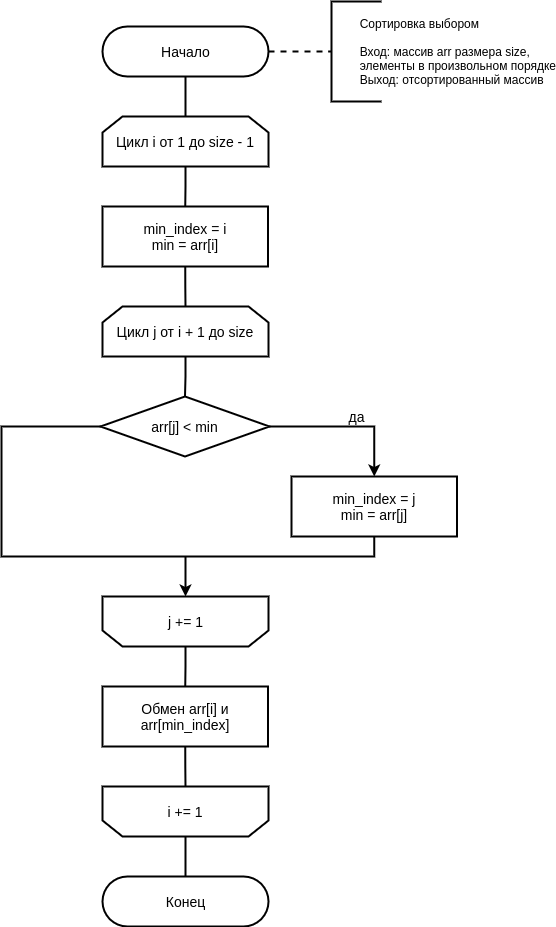
\includegraphics[scale=0.4]{img/selection_sort.png}
	\end{center}
	\captionsetup{justification=centering}
	\caption{Схема алгоритма сортировки выбором}
	\label{img:selection_sort}
\end{figure}

\begin{figure}[H]
	\begin{center}
		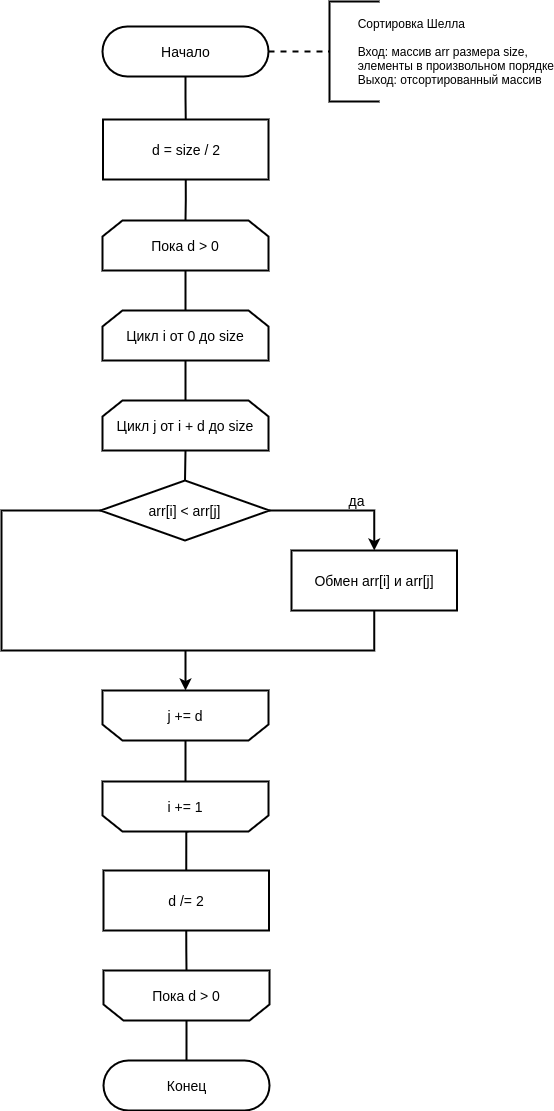
\includegraphics[scale=0.5]{img/shell_sort.png}
	\end{center}
	\captionsetup{justification=centering}
	\caption{Схема алгоритма сортировки Шелла}
	\label{img:shell_sort}
\end{figure}

\newpage

\begin{figure}[H]
	\begin{center}
		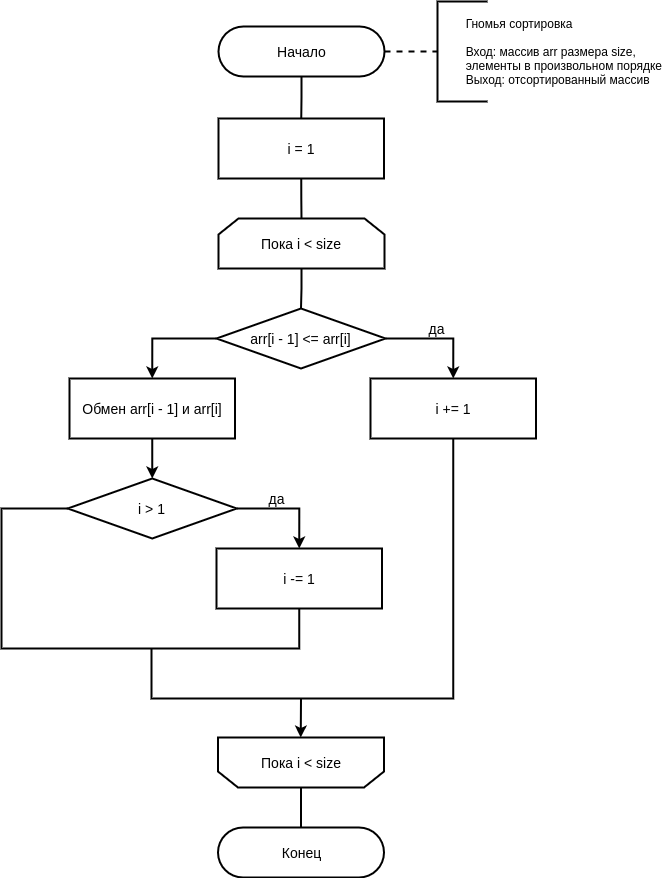
\includegraphics[scale=0.5]{img/gnome_sort.png}
	\end{center}
	\captionsetup{justification=centering}
	\caption{Схема алгоритма гномьей сортировки}
	\label{img:gnome_sort}
\end{figure}

\section*{Вывод}

Были представлены схемы алгоритмов сортировки выбором, Шелла и гномьей сортировки и указаны требования к ПО.

% схемы алгоритмов, типы и структуры данных, все, что сам придумал
\chapter{Технологическая часть}

В данном разделе будут указаны средства реализации, будут представлены листинги кода, а также функциональные тесты.

\section{Средства реализации}

Реализация данной лабораторной работы выполнялась при помощи языка программирования Python \cite{python}. Выбор ЯП обусловлен простотой синтаксиса, большим числом библиотек и эффективностью визуализации данных.

Замеры времени проводились при помощи функции process\_time из библиотеки time \cite{python-time}.

\section{Листинги кода}

Стандартный алгоритм, алгоритм Винограда и оптимизированный алгоритм Винограда умножения матриц приведены в листингах \ref{lst:standard}-\ref{lst:optimized}.

\begin{center}
\captionsetup{justification=raggedright,singlelinecheck=off}
\begin{lstlisting}[label=lst:standard,caption=Стандартный алгоритм умножения матриц]
def standard_mult(A, B):
    n = len(A)
    m = len(B[0])
    p = len(A[0])

    C = [[0] * m for i in range(n)]

    for i in range(n):
        for j in range(m):
            for k in range(p):
                C[i][j] += A[i][k] * B[k][j]

    return C
\end{lstlisting} 
\end{center}
\clearpage
\begin{center}
\captionsetup{justification=raggedright,singlelinecheck=off}
\begin{lstlisting}[label=lst:winograd,caption=Алгоритм Винограда умножения матриц]
def winograd_mult(A, B):
    n = len(A)
    m = len(B[0])
    p = len(A[0])

    C = [[0] * m for _ in range(n)]

    row_factors = [0] * n

    for i in range(n):
        for j in range(p // 2):
            row_factors[i] = row_factors[i] + \
                             A[i][2 * j] * A[i][2 * j + 1]

    column_factors = [0] * m

    for i in range(m):
        for j in range(p // 2):
            column_factors[i] = column_factors[i] + \
                                B[2 * j][i] * B[2 * j + 1][i]

    for i in range(n):
        for j in range(m):
            C[i][j] = -row_factors[i] - column_factors[j]

            for k in range(p // 2):
                C[i][j] = C[i][j] + (A[i][2 * k + 1] + B[2 * k][j]) * \
                                    (A[i][2 * k] + B[2 * k + 1][j])
    
    if p % 2 != 0:
        for i in range(n):
            for j in range(m):
                C[i][j] = C[i][j] + A[i][p - 1] * B[p - 1][j]
    
    return C
\end{lstlisting}
\end{center}
\clearpage
\begin{center}
\captionsetup{justification=raggedright,singlelinecheck=off}
\begin{lstlisting}[label=lst:optimized,caption=Оптимизированный алгоритм Винограда умножения матриц]
def optimized_winograd_mult(A, B):
    n = len(A)
    m = len(B[0])
    p = len(A[0])

    C = [[0] * m for _ in range(n)]

    row_factors = [0] * n

    for i in range(n):
        for j in range(1, p, 2):
            row_factors[i] += A[i][j] * A[i][j - 1]

    column_factors = [0] * m

    for i in range(m):
        for j in range(1, p, 2):
            column_factors[i] += B[j][i] * B[j - 1][i]

    flag = p % 2

    for i in range(n):
        for j in range(m):
            C[i][j] = -(row_factors[i] + column_factors[j])

            for k in range(1, p, 2):
                C[i][j] += (A[i][k - 1] + B[k][j]) * \
                                    (A[i][k] + B[k - 1][j])
    
            if flag:
                C[i][j] += A[i][p - 1] * B[p - 1][j]
    
    return C
\end{lstlisting}
\end{center}

\section{Функциональные тесты}

В таблице \ref{tbl:func_test} приведены функциональные тесты для функций, реализующих алгоритмы умножения матриц. Все тесты пройдены успешно.

\begin{table}[h]
	\begin{center}
		\begin{threeparttable}
		\captionsetup{justification=raggedright,singlelinecheck=off}
		\caption{\label{tbl:func_test} Функциональные тесты}
		\begin{tabular}{|c@{\hspace{7mm}}|c@{\hspace{7mm}}|c@{\hspace{7mm}}|c@{\hspace{7mm}}|c@{\hspace{7mm}}|c@{\hspace{7mm}}|}
			\hline
			Матрица A & Матрица B & Ожидаемый результат \\ 
			\hline
			$\begin{pmatrix}
				&
			\end{pmatrix}$ &
			$\begin{pmatrix}
				&
			\end{pmatrix}$ &
			Сообщение об ошибке \\ \hline

			$\begin{pmatrix}
				&
			\end{pmatrix}$ &
			$\begin{pmatrix}
				1 & 2\\
				3 & 4\\
				5 & 6
			\end{pmatrix}$ &
			Сообщение об ошибке \\ \hline

			$\begin{pmatrix}
				1 & 0 & 1
			\end{pmatrix}$ &
			$\begin{pmatrix}
				-1 & 0 & -1
			\end{pmatrix}$ &
			Сообщение об ошибке \\ \hline

			$\begin{pmatrix}
				1 & 2 & 3 \\
				4 & 5 & 6 \\
				7 & 8 & 9
			\end{pmatrix}$ &
			$\begin{pmatrix}
				-1 & -2 & -3 \\
				-4 & -5 & -6 \\
				-7 & -8 & -9
			\end{pmatrix}$ &
			$\begin{pmatrix}
				-30 & -36 & -42 \\
				-66 & -81 & -96 \\
				-102 & -126 & -150
			\end{pmatrix}$ \\ \hline

			$\begin{pmatrix}
				1 & 2 & 3
			\end{pmatrix}$ &
			$\begin{pmatrix}
				1 \\
				2 \\
				3
			\end{pmatrix}$ &
			$\begin{pmatrix}
				14 \\
			\end{pmatrix}$ \\ \hline

		\end{tabular}
		\end{threeparttable}
	\end{center}
	
\end{table}

\section{Вывод}

Были реализованы функции алгоритмов умножения матриц. Было проведено функциональное тестирование указанных функций.
\chapter{Исследовательская часть}

В данном разделе будут приведены примеры работы программы, и будет проведен сравнительный анализ реализованных алгоритмов сортировки по затраченному процессорному времени.

\section{Технические характеристики}

Тестирование проводилось на устройстве со следующими техническими характеристиками:

\begin{itemize}
	\item операционная система: Ubuntu 20.04.1 Linux x86\_64;
	\item память : 8 GiB;
	\item процессор: AMD® Ryzen™ 3 3200u.
\end{itemize}

Тестирование проводилось на ноутбуке, включенном в сеть электропитания. Во время тестирования ноутбук был нагружен только встроенными приложениями окружения, а также непосредственно системой тестирования.

\section{Демонстрация работы программы}

На рисунке приведен пример работы программы.

\section{Время выполнения алгоритмов}

Функция process\_time из библиотеки time ЯП Python возвращает сумму системного и пользовательского процессорного времени в секундах - значение типа float.

Для замера времени:
\begin{enumerate}
	\item получить значение времени до начала сортировки, затем после её окончания. Чтобы получить результат, необходимо вычесть из второго значения первое;
	\item первый шаг необходимо повторить iters раз, суммируя полученные значения, а затем усреднить результат.
\end{enumerate}

Результаты замеров времени работы алгоритмов в миллисекундах приведены в таблицах \ref{tbl:best}, \ref{tbl:worst}, \ref{tbl:random}.

\begin{table}[h]
	\begin{center}
		\begin{threeparttable}
		\captionsetup{justification=raggedleft,singlelinecheck=off}
		\caption{На входе отсортированный массив}
		\label{tbl:best}
		\begin{tabular}{|c|c|c|c|}
			\hline
			Размер & Выбором & Шелла & Гномья \\
			\hline
  			100 & 0.1872 & 0.4463 & 0.0107 \\ 
 			\hline
  			200 & 0.6648 & 1.5769 & 0.0208 \\ 
 			\hline
  			300 & 1.7652 & 4.2090 & 0.0315 \\ 
 			\hline
  			400 & 2.9205 & 6.5499 & 0.0415 \\ 
 			\hline
  			500 & 4.7658 & 9.9785 & 0.0527 \\ 
 			\hline
  			600 & 6.9592 & 17.5923 & 0.0610 \\ 
 			\hline
  			700 & 9.5135 & 23.0703 & 0.0695 \\ 
 			\hline
  			800 & 12.3131 & 26.6032 & 0.0836 \\ 
 			\hline
  			900 & 15.3724 & 32.2987 & 0.0905 \\ 
 			\hline
 			1000 & 18.7373 & 39.5696 & 0.0996 \\ 
 			\hline
		\end{tabular}
		\end{threeparttable}
    \end{center}
\end{table}

\clearpage

\begin{table}[h]
	\begin{center}
		\begin{threeparttable}
		\captionsetup{justification=raggedleft,singlelinecheck=off}
		\caption{На входе отсортированный в обратном порядке массив}
		\label{tbl:worst}
		\begin{tabular}{|c|c|c|c|}
			\hline
			Размер & Выбором & Шелла & Гномья \\
			\hline
  			100 & 0.2276 & 0.4635 & 1.4289 \\ 
 			\hline
  			200 & 0.8215 & 1.6202 & 5.4438 \\ 
 			\hline
  			300 & 2.1278 & 4.2667 & 12.9537 \\ 
 			\hline
  			400 & 3.5504 & 6.6461 & 23.6392 \\ 
 			\hline
  			500 & 5.6489 & 10.0919 & 37.7889 \\ 
 			\hline
  			600 & 8.3033 & 17.7157 & 55.5283 \\ 
 			\hline
  			700 & 11.2540 & 23.2613 & 77.0185 \\ 
			\hline
  			800 & 14.8231 & 26.7550 & 102.4330 \\ 
 			\hline
  			900 & 18.7517 & 33.3306 & 129.7009 \\ 
 			\hline
 			1000 & 23.4290 & 41.0557 & 161.5674 \\ 
 			\hline
		\end{tabular}
		\end{threeparttable}
    \end{center}
\end{table}

\begin{table}[h]
	\begin{center}
		\begin{threeparttable}
		\captionsetup{justification=raggedleft,singlelinecheck=off}
		\caption{На входе случайный массив}
		\label{tbl:random}
		\begin{tabular}{|c|c|c|c|}
			\hline
			Размер & Выбором & Шелла & Гномья \\
			\hline
  			100 & 0.2079 & 0.4813 & 0.7389 \\ 
 			\hline
  			200 & 0.7309 & 1.7043 & 3.0184 \\ 
 			\hline
  			300 & 1.8340 & 4.3971 & 6.5836 \\ 
 			\hline
  			400 & 3.1248 & 6.9417 & 12.2080 \\ 
 			\hline
  			500 & 4.9933 & 10.3987 & 19.7805 \\ 
 			\hline
  			600 & 7.3488 & 18.3833 & 29.6323 \\ 
 			\hline
  			700 & 10.0685 & 23.9719 & 40.9918 \\ 
 			\hline
  			800 & 13.3175 & 27.9766 & 54.7456 \\ 
 			\hline
  			900 & 17.1284 & 34.7869 & 70.0897 \\ 
 			\hline
 			1000 & 20.7750 & 41.5146 & 87.0879 \\ 
 			\hline
		\end{tabular}
		\end{threeparttable}
    \end{center}
\end{table}

На рисунках \ref{img:best-type}, \ref{img:worst-type}, \ref{img:random-type} приведены графические результаты замеров времени работы сортировок от длины входного массива в трех случаях: на входе отсортированный массив, отсортированный в обратном порядке и массив, заполненный случайным образом.

\begin{figure}[H]
	\begin{center}
		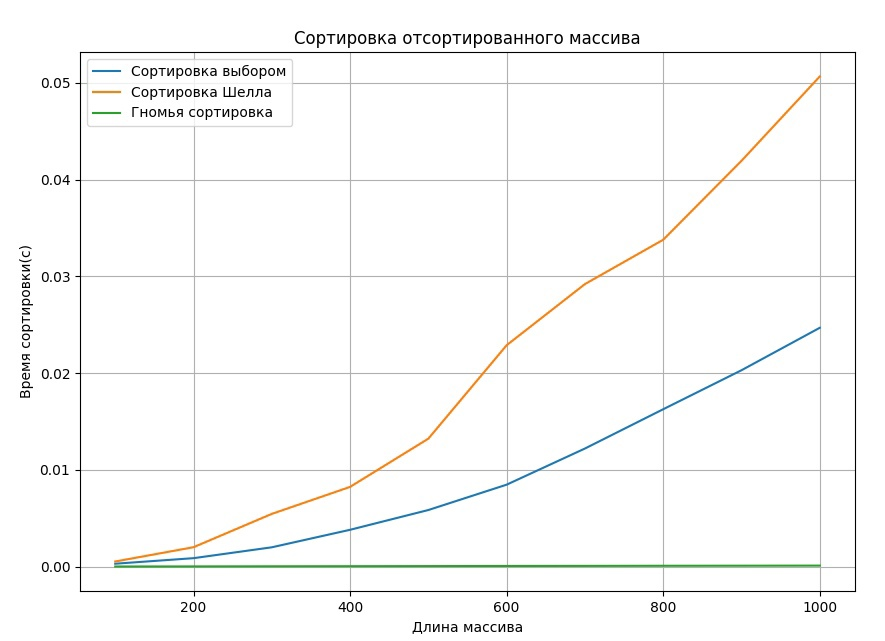
\includegraphics[scale=0.4]{img/best-type.jpg}
	\end{center}
	\captionsetup{justification=centering}
	\caption{На входе отсортированный массив}
	\label{img:best-type}
\end{figure}

\begin{figure}[H]
	\begin{center}
		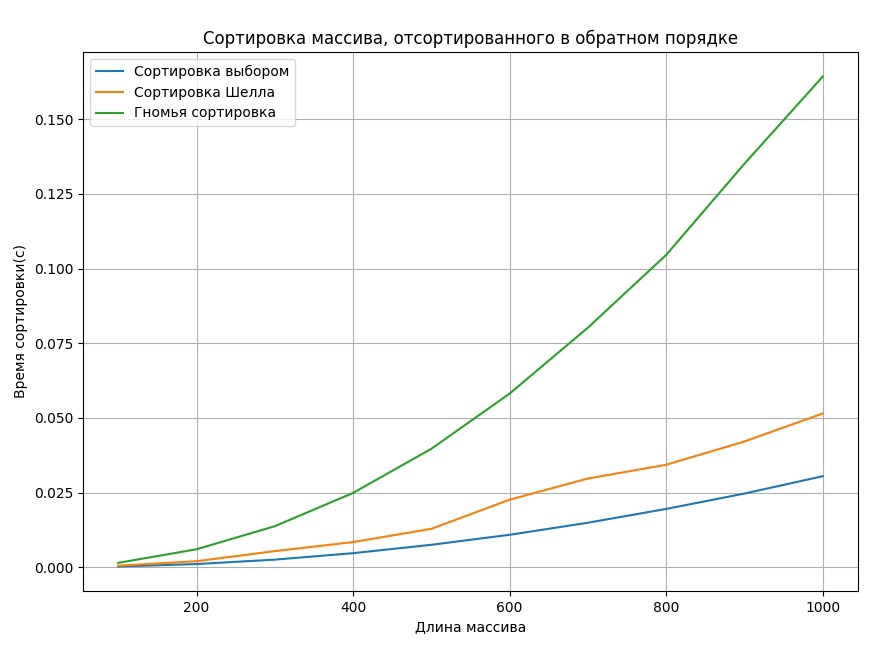
\includegraphics[scale=0.4]{img/worst-type.jpg}
	\end{center}
	\captionsetup{justification=centering}
	\caption{На входе отсортированный в обратном порядке массив}
	\label{img:worst-type}
\end{figure}

\begin{figure}[H]
	\begin{center}
		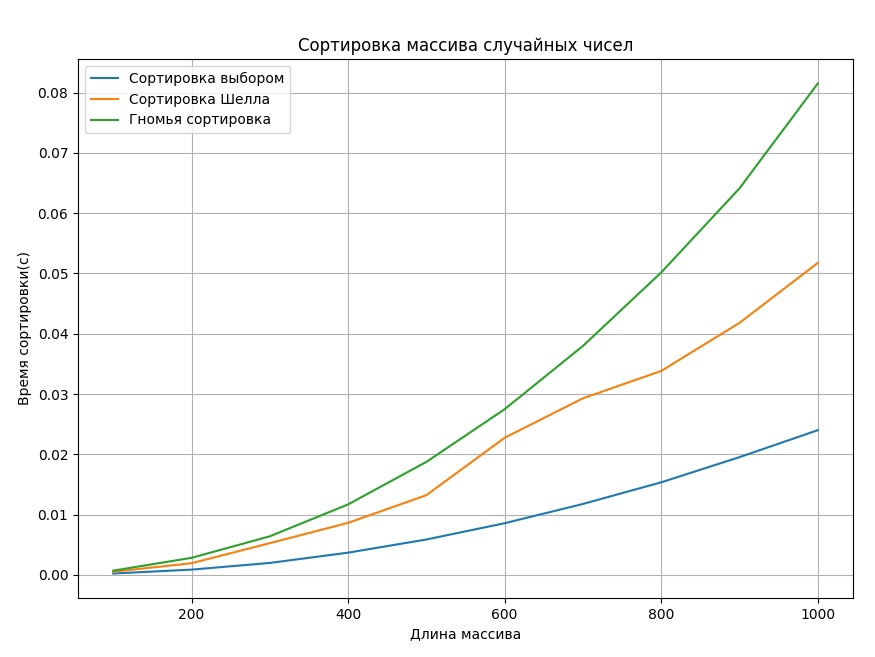
\includegraphics[scale=0.4]{img/random-type.jpg}
	\end{center}
	\captionsetup{justification=centering}
	\caption{На входе заполненный случайно массив}
	\label{img:random-type}
\end{figure}

\section*{Вывод}

Сортировка выбором работает быстрее при сортировке случайно заполненного массива и обратно отсортированного массива. Гномья сортировка в этих случаях работает дольше всех. При этом в случае отсортированного массива гномья сортировка оказывается самой быстрой, самой медленной оказывается сортировка Шелла.
% графики: 10 точек на графике примерно, то есть берём массивы от 10 до 100 с шагом 10 и замеряем по каждому алгоритму время для 3 случаев (лучший, худший, произвольный). Таким образом, 9 графиков для 3 алгоритмов. Здесь же надо указать, как измеряли время (подсказка: нужно замерить одно и то же несколько раз и усреднить).
\chapter*{Заключение}
\addcontentsline{toc}{chapter}{Заключение}

В результате исследования было получено, что при размере матриц, большем 30, небходимо использовать оптимизированный алгоритм умножения матриц по Винограду, так как данный алгоритм работает быстрее стандартного алгоритма в 1.3 раза. При этом стандартный алгоритм медленнее алгоритма Винограда в 1.2 раза.

Кроме того алгоритм Винограда предпочтительно использовать для умножения матриц четных размеров, так как указанный алгоритм работает в 1.2 раза быстрее, чем на матрицах с нечетным размером. Это связано с проведением дополнительных вычислений для крайних строк и столбцов.

Цель, поставленная перед началом работы, была достигнута. В ходе лабораторной работы были решены следующие задачи:

\begin{itemize}
	\item были изучены классический алгоритм, алгоритм Винограда и его оптимизированная версия умножения матриц;
	\item были разработаны изученные алгоритмы;
	\item был проведен сравнительный анализ реализованных алгоритмов;
	\item был подготовлен отчет о выполненной лабораторной работе.
\end{itemize}

\addcontentsline{toc}{chapter}{Литература}
\bibliographystyle{utf8gost705u}
\bibliography{biblio}

\end{document}